\documentclass[conference]{IEEEtran}

\usepackage{fontspec}
\setmainfont{Times New Roman}

\usepackage{cite}
\usepackage[
    colorlinks=true, 
    linkcolor=blue, 
    citecolor=blue,
    urlcolor=blue
]{hyperref}
\usepackage{amsmath,amssymb,amsfonts}
\usepackage{algorithmic}
\usepackage{graphicx}
\usepackage{textcomp}
\usepackage{xcolor}
\def\BibTeX{
    {\rm B\kern-.05em{\sc i\kern-.025em b}\kern-.08em
    T\kern-.1667em\lower.7ex\hbox{E}\kern-.125emX}
}

\usepackage{cuted}
\usepackage{caption}
\usepackage{float}

\begin{document}

\title{Dynamic Scene Modeling and Rendering: A Survey of Methods and Applications}

\author{
    \IEEEauthorblockN{
        Yuwei ZHAO\IEEEauthorrefmark{1},
        Kaiyuan ZHANG\IEEEauthorrefmark{2},
        Yuxiang LIU\IEEEauthorrefmark{3},
        Yilin ZHANG\IEEEauthorrefmark{3},
        Keqin ZHANG\IEEEauthorrefmark{3}
    }

    \\ [0.1pt]

    \IEEEauthorblockA{
        Faculty of Computer Science and Engineering \\
        Ocean University of China
    }
}

\maketitle

\begin{strip}
    \centering
    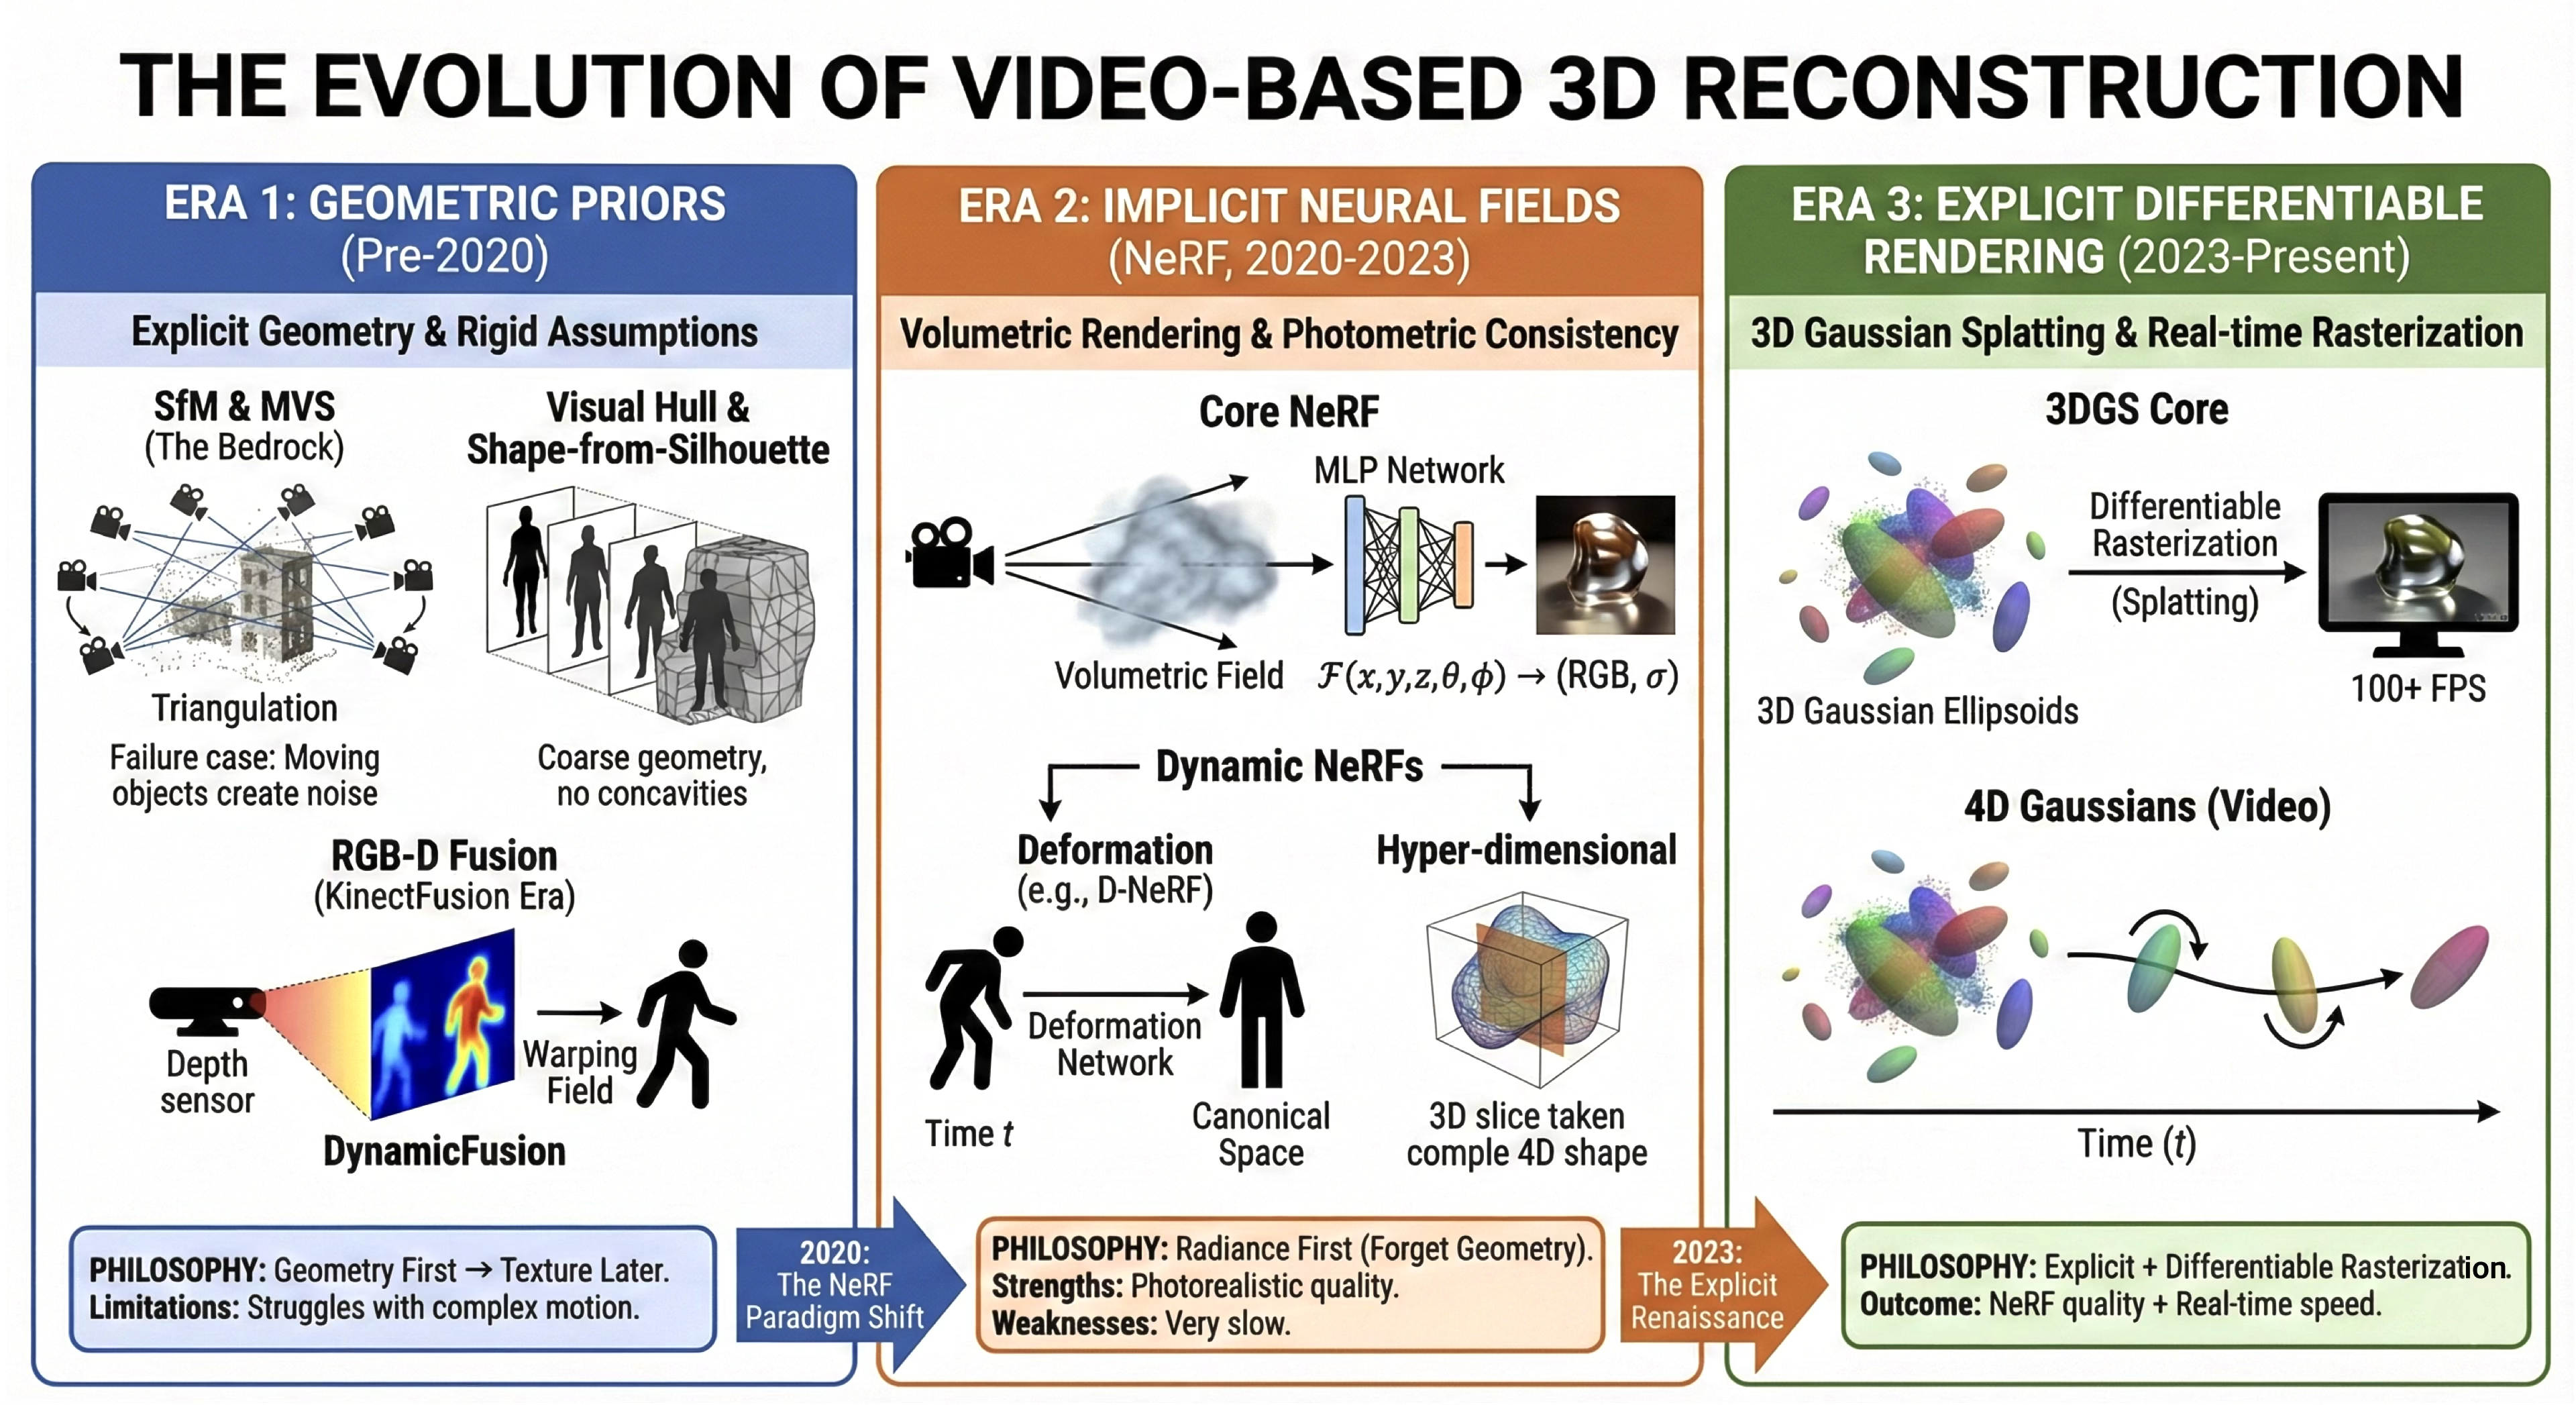
\includegraphics[width=0.9\textwidth]{./img/3d_reconstruction_evolution.png}
    \captionof{figure}{Visualization of the evolution of video-based 3D reconstruction}
    \label{fig:evolution_3d_reconstruction}
\end{strip}

\begin{abstract}
    Dynamic scene modeling and reconstruction from video streams have witnessed a paradigm shift with the advent of Neural Radiance Fields (NeRF) and 3D Gaussian Splatting (3DGS). 
    While NeRF-based methods offer photorealistic quality via implicit neural representations, they often suffer from prohibitive training and rendering costs. 
    Recently, 3DGS has emerged as a powerful alternative, enabling real-time rendering through explicit splatting techniques, though it introduces new challenges regarding storage overhead and temporal consistency. 
    In this paper, we present a comprehensive survey of video-based 3D reconstruction methods, categorizing them into implicit and explicit approaches. 
    We systematically evaluate their trade-offs in terms of rendering quality, speed, and memory consumption across diverse scenarios. 
    Furthermore, we summarize the limitations of current state-of-the-art methods and discuss future directions. 
    Our compiled resources and code are available at \url{https://github.com/8arbatos/Academic-English-Group-Paper}.
\end{abstract}

\begin{IEEEkeywords}
    3D Reconstruction, Dynamic Scene Modeling, Neural Radiance Fields (NeRF), Gaussian Splatting, Novel View Synthesis, Survey.
\end{IEEEkeywords}

\section{Introduction}

\IEEEPARstart{W}{ith} the rapid advancement of virtual reality (VR), augmented reality (AR), and the Metaverse, the demand for photorealistic 3D content creation has surged exponentially. 
Dynamic scene modeling, which aims to reconstruct 3D geometry and appearance from 2D video streams, serves as a fundamental technology for these applications, enabling immersive telepresence, free-viewpoint video, and digital human avatars \cite{intro_metaverse}. 
Unlike static scene reconstruction, modeling dynamic scenes from video presents a highly ill-posed inverse problem due to the entanglement of object motion, topology changes, and time-variant lighting conditions.

Traditionally, 3D reconstruction relied on Structure-from-Motion (SfM) and Multi-View Stereo (MVS) algorithms \cite{colmap}. 
While these methods, such as COLMAP, provide robust camera pose estimation, they struggle to capture thin structures and view-dependent effects (e.g., reflections). 
More importantly, traditional pipelines typically assume a static world, making them brittle when applied to dynamic video sequences where geometry consistency is violated over time.

The field witnessed a paradigm shift with the introduction of \textbf{Neural Radiance Fields (NeRF)} \cite{nerf}. 
By representing scenes as implicit continuous functions parameterized by Multi-Layer Perceptrons (MLPs), NeRF achieved unprecedented rendering quality. 
Subsequent works, such as D-NeRF \cite{dnerf} and Nerfies \cite{nerfies}, extended this implicit paradigm to dynamic domains by introducing deformation fields to handle non-rigid motion. 
However, implicit methods suffer from prohibitive computational costs due to the extensive ray-marching sampling required during both training and inference, limiting their deployment in real-time applications.

Recently, \textbf{3D Gaussian Splatting (3DGS)} \cite{gaussian_splatting} has emerged as a compelling alternative, marking a return to explicit volumetric representations. 
By combining the differentiability of deep learning with the efficiency of rasterization-based rendering, 3DGS enables real-time rendering (100+ FPS) and fast training speeds. 
This breakthrough has triggered a new wave of research focused on extending Gaussian primitives to 4D spatiotemporal modeling \cite{4dgs, dynamic3dgs}, aiming to combine the efficiency of explicit representations with the flexibility of neural fields.

Despite the explosion of research papers in this domain, a systematic comparison between implicit (NeRF-based) and explicit (Gaussian-based) approaches for video modeling is lacking. 
In this survey, we provide a comprehensive review of the state-of-the-art methods for video-based 3D reconstruction. 
The main contributions of this paper are summarized as follows:

\begin{itemize}
    \item We propose a structured taxonomy of dynamic scene modeling methods, categorizing them into \textit{Deformation-based}, \textit{Spacetime-based}, and \textit{Hybrid} approaches across both implicit and explicit representations.
    \item We provide an in-depth analysis of the transition from NeRF to 3D Gaussian Splatting, highlighting the trade-offs between rendering quality, training efficiency, and storage overhead.
    \item We conduct a comparative evaluation of representative frameworks and discuss open challenges, including storage optimization and long-duration video modeling, to guide future research directions.
\end{itemize}

\section{Prepare Your Paper Before Styling}
Before you begin to format your paper, first write and save the content as a 
separate text file. Complete all content and organizational editing before 
formatting. Please note sections \ref{AA} to \ref{FAT} below for more information on 
proofreading, spelling and grammar.

Keep your text and graphic files separate until after the text has been 
formatted and styled. Do not number text heads---{\LaTeX} will do that 
for you.

\subsection{Abbreviations and Acronyms}\label{AA}
Define abbreviations and acronyms the first time they are used in the text, 
even after they have been defined in the abstract. Abbreviations such as 
IEEE, SI, MKS, CGS, ac, dc, and rms do not have to be defined. Do not use 
abbreviations in the title or heads unless they are unavoidable.

\subsection{Units}
\begin{itemize}
\item Use either SI (MKS) or CGS as primary units. (SI units are encouraged.) English units may be used as secondary units (in parentheses). An exception would be the use of English units as identifiers in trade, such as ``3.5-inch disk drive''.
\item Avoid combining SI and CGS units, such as current in amperes and magnetic field in oersteds. This often leads to confusion because equations do not balance dimensionally. If you must use mixed units, clearly state the units for each quantity that you use in an equation.
\item Do not mix complete spellings and abbreviations of units: ``Wb/m\textsuperscript{2}'' or ``webers per square meter'', not ``webers/m\textsuperscript{2}''. Spell out units when they appear in text: ``. . . a few henries'', not ``. . . a few H''.
\item Use a zero before decimal points: ``0.25'', not ``.25''. Use ``cm\textsuperscript{3}'', not ``cc''.)
\end{itemize}

\subsection{Equations}
Number equations consecutively. To make your 
equations more compact, you may use the solidus (~/~), the exp function, or 
appropriate exponents. Italicize Roman symbols for quantities and variables, 
but not Greek symbols. Use a long dash rather than a hyphen for a minus 
sign. Punctuate equations with commas or periods when they are part of a 
sentence, as in:
\begin{equation}
a+b=\gamma\label{eq}
\end{equation}

Be sure that the 
symbols in your equation have been defined before or immediately following 
the equation. Use ``\eqref{eq}'', not ``Eq.~\eqref{eq}'' or ``equation \eqref{eq}'', except at 
the beginning of a sentence: ``Equation \eqref{eq} is . . .''

\subsection{\LaTeX-Specific Advice}

Please use ``soft'' (e.g., \verb|\eqref{Eq}|) cross references instead
of ``hard'' references (e.g., \verb|(1)|). That will make it possible
to combine sections, add equations, or change the order of figures or
citations without having to go through the file line by line.

Please don't use the \verb|{eqnarray}| equation environment. Use
\verb|{align}| or \verb|{IEEEeqnarray}| instead. The \verb|{eqnarray}|
environment leaves unsightly spaces around relation symbols.

Please note that the \verb|{subequations}| environment in {\LaTeX}
will increment the main equation counter even when there are no
equation numbers displayed. If you forget that, you might write an
article in which the equation numbers skip from (17) to (20), causing
the copy editors to wonder if you've discovered a new method of
counting.

{\BibTeX} does not work by magic. It doesn't get the bibliographic
data from thin air but from .bib files. If you use {\BibTeX} to produce a
bibliography you must send the .bib files. 

{\LaTeX} can't read your mind. If you assign the same label to a
subsubsection and a table, you might find that Table I has been cross
referenced as Table IV-B3. 

{\LaTeX} does not have precognitive abilities. If you put a
\verb|\label| command before the command that updates the counter it's
supposed to be using, the label will pick up the last counter to be
cross referenced instead. In particular, a \verb|\label| command
should not go before the caption of a figure or a table.

Do not use \verb|\nonumber| inside the \verb|{array}| environment. It
will not stop equation numbers inside \verb|{array}| (there won't be
any anyway) and it might stop a wanted equation number in the
surrounding equation.

\subsection{Some Common Mistakes}\label{SCM}
\begin{itemize}
\item The word ``data'' is plural, not singular.
\item The subscript for the permeability of vacuum $\mu_{0}$, and other common scientific constants, is zero with subscript formatting, not a lowercase letter ``o''.
\item In American English, commas, semicolons, periods, question and exclamation marks are located within quotation marks only when a complete thought or name is cited, such as a title or full quotation. When quotation marks are used, instead of a bold or italic typeface, to highlight a word or phrase, punctuation should appear outside of the quotation marks. A parenthetical phrase or statement at the end of a sentence is punctuated outside of the closing parenthesis (like this). (A parenthetical sentence is punctuated within the parentheses.)
\item A graph within a graph is an ``inset'', not an ``insert''. The word alternatively is preferred to the word ``alternately'' (unless you really mean something that alternates).
\item Do not use the word ``essentially'' to mean ``approximately'' or ``effectively''.
\item In your paper title, if the words ``that uses'' can accurately replace the word ``using'', capitalize the ``u''; if not, keep using lower-cased.
\item Be aware of the different meanings of the homophones ``affect'' and ``effect'', ``complement'' and ``compliment'', ``discreet'' and ``discrete'', ``principal'' and ``principle''.
\item Do not confuse ``imply'' and ``infer''.
\item The prefix ``non'' is not a word; it should be joined to the word it modifies, usually without a hyphen.
\item There is no period after the ``et'' in the Latin abbreviation ``et al.''.
\item The abbreviation ``i.e.'' means ``that is'', and the abbreviation ``e.g.'' means ``for example''.
\end{itemize}
An excellent style manual for science writers is \cite{b7}.

\subsection{Authors and Affiliations}\label{AAA}
\textbf{The class file is designed for, but not limited to, six authors.} A 
minimum of one author is required for all conference articles. Author names 
should be listed starting from left to right and then moving down to the 
next line. This is the author sequence that will be used in future citations 
and by indexing services. Names should not be listed in columns nor group by 
affiliation. Please keep your affiliations as succinct as possible (for 
example, do not differentiate among departments of the same organization).

\subsection{Identify the Headings}\label{ITH}
Headings, or heads, are organizational devices that guide the reader through 
your paper. There are two types: component heads and text heads.

Component heads identify the different components of your paper and are not 
topically subordinate to each other. Examples include Acknowledgments and 
References and, for these, the correct style to use is ``Heading 5''. Use 
``figure caption'' for your Figure captions, and ``table head'' for your 
table title. Run-in heads, such as ``Abstract'', will require you to apply a 
style (in this case, italic) in addition to the style provided by the drop 
down menu to differentiate the head from the text.

Text heads organize the topics on a relational, hierarchical basis. For 
example, the paper title is the primary text head because all subsequent 
material relates and elaborates on this one topic. If there are two or more 
sub-topics, the next level head (uppercase Roman numerals) should be used 
and, conversely, if there are not at least two sub-topics, then no subheads 
should be introduced.

\subsection{Figures and Tables}\label{FAT}
\paragraph{Positioning Figures and Tables} Place figures and tables at the top and 
bottom of columns. Avoid placing them in the middle of columns. Large 
figures and tables may span across both columns. Figure captions should be 
below the figures; table heads should appear above the tables. Insert 
figures and tables after they are cited in the text. Use the abbreviation 
``Fig.~\ref{fig}'', even at the beginning of a sentence.

\begin{table}[htbp]
\caption{Table Type Styles}
\begin{center}
\begin{tabular}{|c|c|c|c|}
\hline
\textbf{Table}&\multicolumn{3}{|c|}{\textbf{Table Column Head}} \\
\cline{2-4} 
\textbf{Head} & \textbf{\textit{Table column subhead}}& \textbf{\textit{Subhead}}& \textbf{\textit{Subhead}} \\
\hline
copy& More table copy$^{\mathrm{a}}$& &  \\
\hline
\multicolumn{4}{l}{$^{\mathrm{a}}$Sample of a Table footnote.}
\end{tabular}
\label{tab1}
\end{center}
\end{table}

Figure Labels: Use 8 point Times New Roman for Figure labels. Use words 
rather than symbols or abbreviations when writing Figure axis labels to 
avoid confusing the reader. As an example, write the quantity 
``Magnetization'', or ``Magnetization, M'', not just ``M''. If including 
units in the label, present them within parentheses. Do not label axes only 
with units. In the example, write ``Magnetization (A/m)'' or ``Magnetization 
\{A[m(1)]\}'', not just ``A/m''. Do not label axes with a ratio of 
quantities and units. For example, write ``Temperature (K)'', not 
``Temperature/K''.

\section*{Acknowledgment}

The preferred spelling of the word ``acknowledgment'' in America is without 
an ``e'' after the ``g''. Avoid the stilted expression ``one of us (R. B. 
G.) thanks $\ldots$''. Instead, try ``R. B. G. thanks$\ldots$''. Put sponsor 
acknowledgments in the unnumbered footnote on the first page.

\begin{thebibliography}{99}
    \bibitem{intro_metaverse} Apple Inc.
    "EXPRESSION ESTIMATION FOR HEADSETS USING LOW-PROFILE ANTENNA AND IMPEDANCE CHARACTERISTIC SENSING"

    \bibitem{colmap} Johannes Schönberger, Jan-Michael Frahm, Marc Pollefeys, Paul-Edouard Sarlin, and Shaohui Liu,
    "COLMAP"
    [Online]. Available: \url{https://colmap.github.io/index.html}.

    \bibitem{nerf} B. Mildenhall, P. P. Srinivasan, M. Tancik, J. T. Barron, R. Ramamoorthi, and R. Ng, 
    "NeRF: Representing Scenes as Neural Radiance Fields for View Synthesis," arXiv preprint arXiv:2003.08934, 2020.
    [Online]. Available: \url{https://arxiv.org/abs/2003.08934}

    \bibitem{dnerf} Albert Pumarola, Enric Corona, Gerard Pons-Moll, and Francesc Moreno-Noguer,
    "D-NeRF: Neural Radiance Fields for Dynamic Scenes", arXiv preprint arXiv:2011.13961, 2020.
    [Online]. Available: \url{https://arxiv.org/abs/2011.13961}

    \bibitem{nerfies} Keunhong Park, Utkarsh Sinha, Jonathan T. Barron, Sofien Bouaziz, Dan B Goldman, Steven M. Seitz, and Ricardo Martin-Brualla,
    "Nerfies: Deformable Neural Radiance Fields", arXiv preprint arXiv:2011.12948, 2021.
    [Online]. Available: \url{https://arxiv.org/abs/2011.12948}

    \bibitem{gaussian_splatting} J. Kerbl, A. Wang, F. Rousselle, and V. Koltun, 
    "3D Gaussian Splatting for Real-Time Radiance Field Rendering", arXiv preprint arXiv:2304.08914, 2023.
    [Online]. Available: \url{https://arxiv.org/abs/2308.04079}

    \bibitem{4dgs} Guanjun Wu, Taoran Yi, Jiemin Fang, Lingxi Xie, Xiaopeng Zhang, Wei Wei, Wenyu Liu, Qi Tian, and Xinggang Wang,
    "4D Gaussian Splatting for Real-Time Dynamic Scene Rendering", arXiv preprint arXiv:2310.08528, 2024.
    [Online]. Available: \url{https://arxiv.org/abs/2310.08528}

    \bibitem{dynamic3dgs} Jonathon Luiten, Georgios Kopanas, Bastian Leibe, and Deva Ramanan,
    "Dynamic 3D Gaussians: Tracking by Persistent Dynamic View Synthesis", arXiv preprint arXiv:2308.09713, 2023.
    [Online]. Available: \url{https://arxiv.org/abs/2308.09713}
\end{thebibliography}

\end{document}